\subsection{``Just Available''}

As David packed his laptop, he ran the exchange through his head again. What intrigued him were not her words, 
but her cadence. It was the way Mia never pushed, and only suggested. It was the same way Hart never cornered, and only 
invited. It was the way every ``thing'' wasn’t mandatory. It was just... available.

``Is someone entrapping me?'' he thought. ``Or are they just letting me see the menu?''

He paused at the elevator, thumb hovering over the button. 

The thought looped louder: ``Was that really a party invitation? Or a test? Or both?''

But his mind didn’t stop there.

It never did.

He wasn't paranoid. He’d seen it before. In L.A. once. Or maybe Austin.

A private equity partner --- sleek, subtle, and always smiling --- had helped ``introduce'' 
a unicorn to 
the founder of a startup that just so happened to be eating market share from one of his 
portfolio companies.

She was charismatic, strategic, and disarmingly earnest. They met at a retreat. She played the 
long game. Two months in, he trusted her. Three months in, she had access. Four months in, she 
had leverage.

And then came the twist.

Turns out she wasn’t just his. She was being quietly, casually, and consensually
``shared'' with the competitor’s executive team, 
too. 

The PE guys didn’t need threats. They just used her to make suggestions.

Within a year, the competitor pivoted strategy. Fatally.

\medskip

\begin{HistoricalSidebar}{The SoftBank Vision Fund Blackmail Plot (2015)}
  
  In 2015, \textbf{Rajeev Misra}, the head of SoftBank’s Vision Fund, allegedly orchestrated 
  a covert plot to undermine \textbf{Nikesh Arora}, SoftBank’s then-president and a rising 
  star positioned as heir apparent to founder Masayoshi Son.
  
  \medskip
  
  According to multiple reports, Misra hired intermediaries to lure Arora into a compromising 
  situation:  
  
  \medskip
  
  \begin{itemize}
    \item A Tokyo hotel room.
    \item Several women arranged to meet him.
    \item Hidden cameras set up to capture incriminating footage.
  \end{itemize}

  \medskip
  
  The plan?  Use the footage as blackmail—forcing Arora’s resignation and clearing Misra’s 
  path to greater power within the company.
  
  \medskip
  
  But the scheme reportedly failed. Arora never took the bait. The plot came to light only 
  later through internal investigations and media reports.
  
  \medskip
  
  \textbf{The illusion?} A boardroom rivalry won through corporate strategy.
  
  \medskip
  
  \textbf{The reality?} A backroom game of espionage, manipulation, and attempted entrapment.
  
  \medskip
  
  In high-stakes corporate settings, the power struggle isn’t always played out in quarterly 
  reports or press releases. Sometimes it happens in whispered deals, shadowy setups, and 
  schemes designed to destroy not just reputations—but futures.
  
  \begin{quote}
  \textbf{The Lesson?} When the perks start arriving unasked, and the invitations seem too good 
  to be true, it’s not networking. It’s grooming. And the next step might not be a promotion, 
  but a trap.
  \end{quote}
  
\end{HistoricalSidebar}

\medskip

The reason he even knew about the story was because the private equity partners bragged about it.

They were telling it to him like a postmortem with cocktails.

He remembered how one of them leaned back and while swirling his drink said:
``It wasn’t even hard. The unicorn did most of the work.''

Another laughed.
``We didn’t have to hack anything. We just let him think she was loyal.''

They passed around the story like a trophy.

They mentioned how she mirrored the competitor’s founder.

They mentioned how she told them of his insecurities and his ambitions.

They mentioned how they had her give them early drafts of his investor memos, internal slide decks, 
and which buzzwords were landing with their board.

But the real brilliance wasn’t just getting the intel.

It was making him act.

They mentioned how they manipulated him through her.

``She didn’t even have to lie,'' one of them said. ``She just nudged the framing.''

``We fed it to his ego. We let him think it was his insight.'' The other partner interjected.

``He sold it to the board himself,'' another added. ``He closed the pitch with `trust me 
on this.' like he knew what he was doing''

``And they did,'' someone said, smirking. ``All the way into that cliff.''

It wasn’t the act that shocked David.

It was the audacity... and the arrogance... and the utter lack of shame.

They didn’t whisper.

They didn’t flinch.

And they didn't care.

Because for them, it wasn’t immoral.

It was strategy.

\medskip

\begin{HistoricalSidebar}{Cambridge Analytica and the Corporate Playbook of Political Manipulation}

    In 2018, undercover footage revealed Cambridge Analytica executives discussing how 
    they could entrap political figures using \textbf{honey traps, bribery stings, and 
    fake news campaigns} \cite{guardian2018}. These tactics were presented not as outliers 
    but as part of a service portfolio designed to shape political outcomes across the globe.
    
    \medskip
    
    The executives—most notably CEO Alexander Nix—boasted about strategies that included sending 
    ``beautiful Ukrainian girls'' to a rival candidate’s house, staging bribery stings, and 
    disseminating false information online \cite{wired2018}. They framed these tactics as 
    standard offerings to clients seeking to influence political landscapes.
    
    \medskip
    
    Despite the public drama, no conclusive evidence emerged that the company \textbf{successfully 
    blackmailed} any specific political figure using these methods. Cambridge Analytica insisted 
    the executives were merely playing along with a hypothetical client to test their 
    intentions \cite{axios2018}. Still, the scandal underscored a chilling trend in modern politics:
    
    \begin{quote}
    In the age of big data, politics isn't just about policies or popularity.  
    It's about manipulation—and the tools aren't just digital. They're deeply personal.
    \end{quote}
    
    \begin{thebibliography}{9}
    \bibitem{guardian2018}
    The Guardian, \textit{Cambridge Analytica Executives Boast of Dirty Tricks to Swing Elections}, 
    March 19, 2018. 
    \url{https://www.theguardian.com/uk-news/2018/mar/19/cambridge-analytica-execs-boast-dirty-tricks-honey-traps-elections}
    
    \bibitem{wired2018}
    WIRED, \textit{Cambridge Analytica Execs Caught Discussing Extortion and Fake News}, March 20, 2018. 
    \url{https://www.wired.com/story/cambridge-analytica-execs-caught-discussing-extortion-and-fake-news/}
    
    \bibitem{axios2018}
    Axios, \textit{Cambridge Analytica Responds to Channel 4 Claims: They Were Entrapped}, March 19, 2018. 
    \url{https://www.axios.com/2018/03/19/cambridge-analytica-responds-to-channel-4-claims-they-were-entrapped}
    \end{thebibliography}
    
\end{HistoricalSidebar}

\medskip

He started running scenarios in his head:

\begin{itemize}
    \item \textbf{If she’s operating solo, this is a flirtation.}
    That would make it personal — unpredictable, maybe risky, but navigable. A matter of emotional dynamics, not institutional politics.

    \item \textbf{If she’s part of something bigger, it’s positioning.} 
    Then it’s not about her at all. It’s about signaling, influence, or soft coercion — part of a wider choreography with him as the data point.

    \item \textbf{If he says yes, he signals openness.} 
    That could be read as consent — not just to her, but to whoever’s watching. A willingness to play, to bend, to be pliable. A future liability in the form of trust.

    \item \textbf{If he says no, he risks signaling disloyalty.} 
    Because refusal isn’t neutral. Refusal can look like resistance. And resistance — in the wrong game — can be logged, archived, and interpreted as a threat.
\end{itemize}


``Assume asymmetric information,'' he muttered silently. ``Assume multiple actors.''

Then he ran the simulation in his head.

\begin{tcolorbox}[
    enhanced,
    sharp corners,
    boxrule=0pt,
    colback=gray!3,
    borderline west={2pt}{0pt}{gray!60}, % vertical bar on the left
    left=10pt,
    right=10pt,
    top=6pt,
    bottom=6pt,
    width=\linewidth,
    fontupper=\small\itshape
  ]
Not everyone in the room knows the same thing.
Not everyone in the room wants the same thing.
Some are watching the game.
Some are playing it.
And some are the game.

\medskip

If Mia was solo, that was one kind of risk.
If Mia was reporting upward, that was another.
If she wasn’t reporting at all --- but just signposting to someone else --- I wouldn’t 
even know which moves were being logged.

\medskip

I have to consdier layered actors. 
And I have to consider nested objectives.

\medskip

That’s what makes this hard.

\medskip

Because even if I make the right move...
It could still be the wrong game.

\medskip

Maybe she didn’t need me to say yes.
Maybe she just needed to see how long I paused before saying no.

\medskip

Maybe my hesitation was the data.

\medskip

Maybe the real question wasn’t what’s on offer
but who’s doing the offering... and who’s watching the table.

\end{tcolorbox}

When he entered the elevator, the air was thick with that faint citrus and rosemary scent 
from the rooftop. 

Now, standing in the elevator, David analyzed Mia’s phrasing.

\textbf{Her cadence} was measured, but never mechanical.
She let silence do half the talking. She never rushing to fill the gaps.
Every phrase landed like it had already been edited twice.
She didn’t interrupt, but she also never waited too long.
She used just enough rhythm to suggest confidence.
She used just enough space to invite projection.


\textbf{Her timing} was impeccable, but plausible.
She didn’t ask questions. She left openings.
She didn't leave opening when things were loud, but when things were quiet
and when the energy softened.
She knew when to make eye contact. 
She knew when to look away. 
She knew when to ask something that felt spontaneous but was clearly sequenced.
She acted like a magician who lets you pick the card—but only after you've already decided.

\textbf{Her restraint} was the most unnerving part.
She was never pressing. Instead, she leaning in. She left no hint of need.
She didn’t reach for the next step. She just left the next step visible.
She just acted like there was a path that had always been there.
She never implied urgency.
She implied inevitability.

Then he ran the simulation again.

\begin{tcolorbox}[
    enhanced,
    sharp corners,
    boxrule=0pt,
    colback=gray!3,
    borderline west={2pt}{0pt}{gray!60}, % vertical bar on the left
    left=10pt,
    right=10pt,
    top=6pt,
    bottom=6pt,
    width=\linewidth,
    fontupper=\small\itshape
  ]
This was not seduction in the classic sense.

\medskip

Her seduction was something quiet.

\medskip

Her seduction was something nuanced.

\medskip

It was like she didn’t need to close the deal.

\medskip

It was like she was trying to make sure I believed it was my idea.

\medskip

Am I being watched?

\medskip

Or maybe... I'm being tested. 

\medskip

Maybe she's just running someone else's protocol.

\medskip

Is someone trying to corner me?

\medskip

Maybe this isn't about me at all.

\end{tcolorbox}

\medskip

\begin{TechnicalSidebar}{Signaling Games --- When Actions Speak Louder Than Truth}

    In game theory, a \textbf{game} is a formal model of strategic interaction among rational agents. 
    Each player chooses actions from a set of possible moves, aiming to maximize their payoff, 
    given their beliefs about what other players might do.

    \medskip
    
    Games are defined by:

    \medskip

    \begin{itemize}
      \item \textbf{Players:} Who is involved in the decision-making?
      \item \textbf{Actions:} What choices are available to each player?
      \item \textbf{Payoffs:} What are the rewards or penalties for each combination of actions?
      \item \textbf{Information:} What does each player know at each stage of the game?
    \end{itemize}

    \medskip
    
    In many real-world situations, players do not share the same information. 
    This is called \textbf{asymmetric information} — a condition that gives rise to 
    \emph{signaling games}.
    
    \medskip
    
    \textbf{Signaling games} model interactions in which one party (the ``sender'') has private 
    information and chooses an action (a ``signal'') to convey, obscure, or manipulate what 
    another party (the ``receiver'') believes. The receiver then takes an action based on the 
    signal and their own strategic interpretation.
    
    \medskip
    
    Key elements of a signaling game:

    \medskip

    \begin{itemize}
      \item The \textbf{sender} knows something the receiver doesn't (e.g., intent, loyalty, competence).
      \item The \textbf{sender chooses a signal} — often an observable action or behavior.
      \item The \textbf{receiver interprets the signal} and responds — potentially misinterpreting it.
    \end{itemize}

    \medskip
    
    Signals can be:

    \medskip

    \begin{itemize}
      \item \textbf{Costly:} difficult to fake, like effort or sacrifice.
      \item \textbf{Cheap talk:} easy to produce but hard to trust.
      \item \textbf{Separating:} clearly distinguish between types of senders.
      \item \textbf{Pooling:} make all senders look the same.
    \end{itemize}
    
    \medskip
    
    In corporate, romantic, or political settings, signaling games explain why people don’t just say 
    what they mean because direct communication can be manipulated, while behavior, timing, and restraint 
    often carry more reliable signals.

    \medskip
    
    
    In David’s case, Mia’s cadence, restraint, and invitations are not random — 
    they are signals. But of what? And for whom? 
    In a signaling game, even \emph{hesitation} becomes a move.  
    
\end{TechnicalSidebar}

\medskip

David had learned about Higher-Order Beliefs in graduate school.

Not from some glossy case study, but from a fractal-looking game tree that took up half 
the whiteboard and three hours to explain.  The kind of diagram that made normal people 
nauseous and made David... curious.

\medskip

\begin{TechnicalSidebar}{Higher-Order Beliefs: Reasoning Beyond the First Move}

    In strategic environments, it’s not enough to model what another agent wants.  
    You have to model what they think \textit{you} want.  
    And sometimes what they think \textit{you think they want}.
    
    \medskip
    
    These recursive structures are called \textbf{higher-order beliefs}. At base level:
    
    \medskip
    
    \begin{itemize}
      \item \textbf{First-order belief:} I believe that you want X.
      \item \textbf{Second-order belief:} I believe that you believe I want Y.
      \item \textbf{Third-order belief:} I believe that you believe that I believe you want Z.
    \end{itemize}

    \medskip
    
    And so on.
    
    \medskip
    
    In theory, this nesting can go infinitely deep.  
    In practice, humans cap out after 2–3 layers before substituting with heuristics or collapsing 
    the tree into a gut feeling.  
    But elite negotiators, intelligence operatives, and certain types of psychopaths may reason 
    deeper.
    
    \medskip
    
    \textbf{Why it matters:}  
    In game theory, higher-order beliefs determine outcomes in environments of \emph{strategic 
    uncertainty}, where success depends not just on your choices, but on how others model your choices.
    
    \medskip
    
    \textbf{Example:} In poker, a player might bluff (\textit{1st-order deception}), expecting the 
    opponent to call (\textit{2nd-order anticipation}), only to triple-bluff knowing the opponent 
    knows they bluff (\textit{3rd-order reversal}).
    
    \medskip
    
    \textbf{Key risk:}  
    The deeper you go, the less you're predicting reality — and the more you're predicting other 
    people predicting your predictions.  
    Eventually, it stops being strategy and becomes simulation.
    
\end{TechnicalSidebar}

\medskip


It started simple — inference.

"I think she wants something."

That was just an observation. A guess. Harmless.

But David caught himself thinking further.

“Okay, but what does she want?”

“Attention? Reassurance? Leverage?”

Then the quiet justification came.

“I’m not judging. I’m just mapping the terrain.”

But it didn’t stop there.

“If she wants something… that means she’s already considered how I’ll respond.”

“Which means she’s already shaped how she’ll present it.”

“Which means this interaction isn’t neutral — it’s strategic.”

“Which means I should be strategic too.”

He exhaled, not out loud.

“I’m not being manipulative. I’m just staying ahead of the frame.”

But he knew — deep down — what was really happening.

He wasn’t just inferring.

He was constructing her.

Building a working model of her intent, her constraints, her next move — not to understand her better, but to preempt her. To control the emotional geometry of the moment.

“This is empathy,” he told himself again.

Then quieter:

“No... this is architecture.”

And once you start drawing blueprints of someone else’s mind, it’s hard to remember where their walls end and yours begin.

\medskip

\begin{table}[H]
  \centering
  \renewcommand{\arraystretch}{1.6}
  \begin{tabular}{>{\raggedright\arraybackslash}p{3.5cm} 
                  >{\raggedright\arraybackslash}p{5.5cm} 
                  >{\raggedright\arraybackslash}p{5.5cm}}
  \toprule
  \textbf{David’s Strategy} 
  & \textbf{She is Sincere}
  & \textbf{She is Strategic}\\
  \ 
  &
  (authentic, open, not calculating) 
  &
  (calculated, signaling, managing perception) \\

  \midrule
  
  \textbf{Empathetic} \\
  (assumes sincerity, reads emotions generously) 
  
  & \textbf{\faCheck\ Trust builds} \newline
  They connect. Vulnerability meets safety. \newline
  \textit{Outcome: Human intimacy. Low control, high authenticity.}
  
  & \textbf{\faTimes\ Exploited} \newline
  She frames the narrative, uses his openness. \newline
  \textit{Outcome: Emotional vulnerability weaponized.} \\
  
  \midrule
  
  \textbf{Strategic} \\ 
  (models her intent, assumes performance)
  
  & \textbf{\faTimes\ Misread} \newline
  He projects motive where there is none. Trust collapses. \newline
  \textit{Outcome: Distance, defensiveness, self-fulfilling coldness.}
  
  & \textbf{\faGavel\ Mutual performance} \newline
  Each watches the other watch. High control, no intimacy. \newline
  \textit{Outcome: Simulation. Neither loses, but no one lands.} \\
  
  \bottomrule
  \end{tabular}
  \caption{Meta-Strategy Payoff Matrix: Modeling Belief, Sincerity, and Strategic Response}
\end{table}


\medskip

Then it shifted — projection.

"She thinks I want something."

David paused.

“Did she say that?”

No.

“Did she imply it?”

Not exactly.

But it felt true.
Because if he were in her position, that’s what he’d think.

“If someone acted the way I just did — I’d assume they wanted something.”

“So she must be thinking that.”

“She has to be.”

Then came the flip.

“Which means she’s already cautious.”

“Which means I need to manage that perception.”

“Which means I should pull back — or lean in — or frame it differently.”

He blinked once, slow.

“I’m not projecting. I’m modeling.”

But the voice in his head didn’t buy it.

“No — you’re rehearsing her thoughts inside your own. You’re turning your instincts into her intent.”

“You’re not observing her. You’re replacing her.”

That’s the trick of projection:
It doesn’t feel like assumption.
It feels like insight.

But insight built on your own reflection isn’t awareness.
It’s an echo.

And David, in that moment, was no longer seeing her clearly.
He was watching himself... in disguise.

\medskip

\begin{table}[H]
  \centering
  \renewcommand{\arraystretch}{1.6}
  \begin{tabular}{>{\raggedright\arraybackslash}p{7cm} 
                  >{\raggedright\arraybackslash}p{7cm}}
  \toprule
  \textbf{David’s Thought Process (Projection)} & \textbf{Reality / Uncertainty} \\
  \midrule

  \textit{"She thinks I want something."} & No signal received. She said nothing. \\
  \textit{"If I were her, I’d assume that."} & True — but that’s his logic, not hers. \\
  \textit{"She must be cautious."} & Possibly — but inferred without evidence. \\
  \textit{"I need to manage that perception."} & Managing a mirror of himself. \\
  \textit{"I’m not projecting. I’m modeling."} & Actually: modeling himself through her imagined perspective. \\
  \textit{"She’s thinking about what I’m thinking."} & Self-reinforcing loop. No confirmation. \\
  \textbf{Result:} Echo mistaken for signal. & \textbf{Effect:} Loss of clarity. Simulation replaces observation. \\
  
  \bottomrule
  \end{tabular}
  \caption{Projection vs. Perception: When Insight Becomes Echo}
\end{table}

\medskip

Then it layered — inference nested inside inference.

“She thinks I think she wants something.”

David froze.

“Okay. So she sees the shift. She feels me noticing.”

“And now she’s calibrating — because she doesn’t want to appear like she wants something.”

“Which means she’s trying to look neutral. Or effortless. Or casual.”

He leaned back slightly, just enough to create space — not in the room, but in the pattern.

“Which means she knows I’m watching for motive.”

“Which means I need to pretend I’m not.”

“Which means I’m not just managing her perception of me — I’m managing her perception of my perception of her.”

His chest stayed still, but his thoughts didn’t.

“I’m not in a conversation. I’m in a recursive model collapse.”

“Belief... about belief... about belief.”

“Inference eating its own tail.”

He tried to snap out of it.

“Just be present,” he told himself. “Just be real.”

But that was the problem.

By the time you’re modeling someone else’s model of your model?

You’ve already left the moment.

You’re not talking to her anymore.

You’re talking to your simulation of her expectations — and calling it reality.

Then it layered — inference nested inside inference.

“She thinks I think she wants something.”

David froze.

“Okay. So she sees the shift. She feels me noticing.”

“And now she’s calibrating — because she doesn’t want to appear like she wants something.”

“Which means she’s trying to look neutral. Or effortless. Or casual.”

He leaned back slightly, just enough to create space — not in the room, but in the pattern.

“Which means she knows I’m watching for motive.”

“Which means I need to pretend I’m not.”

“Which means I’m not just managing her perception of me — I’m managing her perception of my perception of her.”

His chest stayed still, but his thoughts didn’t.

“I’m not in a conversation. I’m in a recursive model collapse.”

“Belief... about belief... about belief.”

“Inference eating its own tail.”

He tried to snap out of it.

“Just be present,” he told himself. “Just be real.”

But that was the problem.

By the time you’re modeling someone else’s model of your model?

You’ve already left the moment.

You’re not talking to her anymore.

You’re talking to your simulation of her expectations — and calling it reality.

\medskip

\begin{table}[H]
  \centering
  \renewcommand{\arraystretch}{1.6}
  \begin{tabular}{>{\raggedright\arraybackslash}p{7cm} 
                  >{\raggedright\arraybackslash}p{7cm}}
  \toprule
  \textbf{Nested Inference Loop (David’s Internal Logic)} 
  & \textbf{Consequences / Structural Loss} \\
  \midrule

  \textit{“She thinks I think she wants something.”} 
  & Layer 1: First-level recursive intent attribution begins. \\
  
  \textit{“She sees me noticing.”}
  & David assumes she is aware of his inference — perspective shift begins. \\

  \textit{“She’s calibrating — trying to look casual.”} 
  & Observable behavior now reinterpreted through imagined motive. \\

  \textit{“She knows I’m watching for motive.”} 
  & Assumes she is actively modeling him — entering recursive symmetry. \\

  \textit{“I need to manage her perception of my perception of her.”} 
  & David begins performing to a simulation of her simulation of him. \\

  \textit{“I’m in a recursive model collapse.”} 
  & Direct awareness replaced by self-referential logic spiral. \\

  \textit{“Inference eating its own tail.”} 
  & Meta-awareness outpaces presence. Feedback loop detaches from input. \\

  \textbf{Core realization:} \textit{“You’re not talking to her anymore.”} 
  & Final collapse. Engagement becomes simulation. Dialogue becomes rehearsal. \\

  \bottomrule
  \end{tabular}
  \caption{Recursive Inference Collapse: When Belief Displaces Reality}
\end{table}

\medskip




Then it folded — deception disguised as ignorance.

“She thinks I think she doesn’t want anything... because she actually does.”

David didn’t hear those words.
He constructed them — like pressure behind a closed door.

“She’s not denying intent. She’s curating absence.”

“She’s not just withholding. She’s performing emptiness.”

“She knows I read subtext. So she’s feeding me the blank space.”

His jaw flexed — just enough to register the tension.

“She’s betting I’ll see the lack of desire as strategic.”

“Which means the silence isn’t honesty. It’s bait.”

“And if I act on it, I confirm her theory. If I ignore it, I miss the signal.”

“She’s not hiding motive. She’s hiding proof of motive.”

He almost laughed.

“This isn’t conversation anymore. It’s theater.”

But the moment didn’t feel performative. It felt... precise.

“She’s not just deceiving me. She’s counting on me decoding the deception — but still playing along.”

“Because if I call it out, I lose the trust.”

“And if I don’t... I validate the performance.”

That’s the trick of strategic ignorance:
It’s not the absence of truth.
It’s the orchestration of doubt.

And David couldn’t tell anymore if he was following the cues —
or being cued to follow.

\medskip

\begin{table}[H]
  \centering
  \renewcommand{\arraystretch}{1.6}
  \begin{tabular}{>{\raggedright\arraybackslash}p{6.5cm} 
                  >{\raggedright\arraybackslash}p{7.5cm}}
  \toprule
  \textbf{Surface Signal / Absence} 
  & \textbf{David’s Interpretation (Structural Reading)} \\
  \midrule

  \textit{She says nothing.}  
  & She’s curating silence. Not avoiding motive — curating its invisibility. \\

  \textit{She doesn’t ask for anything.} 
  & Performance of emptiness. A negative space designed to be decoded. \\

  \textit{She appears casual, neutral, effortless.} 
  & Intentional posture. Strategic ignorance — crafted to deflect attention while implying depth. \\

  \textit{There’s no accusation, no desire, no reveal.} 
  & The absence *is* the message. Designed ambiguity. Bait. \\

  \textit{David feels pressure to act, or to withhold.} 
  & He's caught in the double-bind: act and confirm her model; don’t act and appear oblivious. \\

  \textit{If he calls it out, he breaks the illusion.} 
  & He risks appearing paranoid or accusatory — losing trust. \\

  \textit{If he plays along, he validates the game.} 
  & He becomes a participant in a script written by implication. \\

  \textbf{Summary:} Silence as structure.  
  & \textbf{Outcome:} Communication shifts from expression to orchestration. Intent is disguised by its own omission. \\

  \bottomrule
  \end{tabular}
  \caption{Strategic Ignorance: Interpreting Absence as a Structured Signal}
\end{table}

\medskip





Then came the loop — recursive inference spiraled through multiple actors.

“She knows I think she wants me to think she’s not thinking about what I’m thinking.”

David blinked — not confusion, but overload.

“She’s not just tracking me. She’s tracking my tracking of her tracking of me.”

“She’s folding intention inside plausible deniability.”

“She wants to seem unaware… but not actually be unaware… just barely plausible enough to keep the ambiguity alive.”

He tried to breathe evenly.

“She’s signaling restraint so I’ll interpret it as self-control, not disinterest.”

“She knows I see the game, so she’s simulating not playing it—just enough to make me second-guess whether she’s in it at all.”

“Which means she’s playing it better than I am.”

A flicker of doubt cracked through.

“Am I mapping her thoughts…”

“Or hallucinating my own?”

“Am I observing… or narrating?”

“Is this mutual perception… or self-reference with a mirror?”

By this point, the model wasn’t layered — it was recursive.

A loop of minds modeling minds until the boundary between actor and observer disappeared.

And David, once so certain of her signal, could no longer tell if he was reading her...

...or just drowning in reflections of himself.

\medskip

\begin{table}[H]
  \centering
  \renewcommand{\arraystretch}{1.6}
  \begin{tabular}{>{\raggedright\arraybackslash}p{7cm} 
                  >{\raggedright\arraybackslash}p{7cm}}
  \toprule
  \textbf{Recursive Mental Model (David’s Perspective)} 
  & \textbf{Effect on Perception / Reality} \\
  \midrule

  \textit{“She knows I think she wants me to think she’s not thinking about what I’m thinking.”} 
  & Full multi-agent recursion begins. Layered belief loops obscure original intent. \\

  \textit{“She’s tracking my tracking of her tracking me.”} 
  & Self-modeling through imagined observer collapses perspective into simulation. \\

  \textit{“She folds intention inside plausible deniability.”} 
  & Signals are deliberately ambiguous — impossible to confirm or deny. \\

  \textit{“She simulates not playing the game, just enough for me to doubt the game exists.”} 
  & Uncertainty becomes a weapon. Her silence is now recursive camouflage. \\

  \textit{“She’s signaling restraint to look like self-control, not disinterest.”} 
  & Emotional ambiguity is interpreted as layered intention. All interpretations remain unprovable. \\

  \textit{“She’s playing it better than I am.”} 
  & Strategic collapse: David feels outmaneuvered in a game with no board. \\

  \textit{“Am I mapping her thoughts… or hallucinating my own?”} 
  & Recursive modeling detaches from any verifiable input. Echo chamber effect. \\

  \textit{“Is this observation or narration?”} 
  & David begins doubting his own internal compass. Signal indistinguishable from story. \\

  \textbf{Conclusion:} \textit{“I’m drowning in reflections of myself.”} 
  & Full epistemic collapse. No longer in dialogue — only in recursive self-reference. \\

  \bottomrule
  \end{tabular}
  \caption{Perception Loop Collapse: Recursive Modeling Across Minds Without Ground Truth}
\end{table}





\medskip






And finally — full recursion with no ground truth.

“She knows that I know that she knows that I want her to think I don’t know.”

David felt the sentence loop in his mind like a Möbius strip — no beginning, no edge, no exit.

“This isn’t strategy anymore.”

“This is simulation.”

He wasn’t analyzing a person. He was running models on top of models, each one reflecting another.

“She’s not responding to me.
She’s responding to my avatar in her head.”

“And I’m responding to her avatar of me in her head… inside my head.”

His chest tightened — not with anxiety, but with uncertainty so dense it felt like fog.

“Where is she in all of this?”

“What does she actually want?”

Silence.

And then, the harder question:

“When did I stop asking?”

Because at this level, not knowing wasn’t a flaw. It was structure.

“Ignorance isn’t an absence. It’s a shield.”

“A way to act without accountability.”

“If I don’t know what she knows, and she doesn’t know what I know—
then neither of us ever has to own the next move.”

It was elegance by erasure.

“No admission. No assertion. Just recursive permission loops.”

“Deniability disguised as complexity.”

He tried to land somewhere — a thought, a fact, a feeling — but there was no ground.

Only inference without anchor. Intention without ownership.

And a quiet realization:

“The moment you stop asking what’s true—”

“—is the moment you become part of the performance.”

\medskip

\begin{table}[H]
  \centering
  \renewcommand{\arraystretch}{1.6}
  \begin{tabular}{>{\raggedright\arraybackslash}p{7cm} 
                  >{\raggedright\arraybackslash}p{7cm}}
  \toprule
  \textbf{Recursive Simulation (David’s Internal Logic)} 
  & \textbf{Collapse of Grounded Perception} \\
  \midrule

  \textit{“She knows that I know that she knows that I want her to think I don’t know.”} 
  & Complete epistemic recursion. Truth displaced by plausible meta-strategy. \\

  \textit{“This isn’t strategy anymore. This is simulation.”} 
  & Simulation becomes the mode of engagement — not a tactic, but a system. \\

  \textit{“She’s responding to my avatar in her head.”} 
  & Dialogue displaced by character interaction between projected selves. \\

  \textit{“I’m responding to her avatar of me in her head… inside my head.”} 
  & Infinite regress. No longer reacting to her — reacting to his own internal simulation. \\

  \textit{“Where is she in all of this?”} 
  & Subject erasure. She becomes unreachable beneath nested abstraction. \\

  \textit{“When did I stop asking?”} 
  & The inquiry into truth was replaced by the rehearsal of impression. \\

  \textit{“Ignorance isn’t absence. It’s a shield.”} 
  & Lack of knowledge becomes a feature — not a flaw — enabling unaccountable maneuvering. \\

  \textit{“No admission. No assertion. Just recursive permission loops.”} 
  & Both parties maintain plausible deniability through mutual ambiguity. \\

  \textbf{Final realization:} \textit{“The moment you stop asking what’s true… is the moment you become part of the performance.”} 
  & Collapse complete. Authenticity is traded for strategic simulation. Presence becomes performance. \\

  \bottomrule
  \end{tabular}
  \caption{Simulation Collapse: When Recursive Modeling Replaces Truth With Performance}
\end{table}

\medskip

\begin{TechnicalSidebar}{Reasoning Types in Multi-Agent Strategic Environments}

    Strategic reasoning in social settings often involves recursive thinking — beliefs about others' beliefs. But the \emph{type} of reasoning matters just as much as the depth. Below are four distinct modes of mental modeling commonly encountered in game-theoretic and psychological contexts:
    
    \medskip

    \begin{itemize}
    
        \item \textbf{Inference:} Agent A forms a belief about Agent B’s desires, intentions, or knowledge state, based on observed behavior. This is the backbone of strategic decision-making: “I think she wants something.”
        \item \textbf{Projection:} Agent A assumes Agent B is motivated by the same desires, fears, or logic that Agent A would possess in the same situation. This can lead to false symmetry: “If I were in her position, I’d do X — so she must want X.”
        \item \textbf{Deception:} Agent A intentionally behaves in a way that creates a false belief in Agent B. This is strategic misrepresentation, often used to gain advantage while masking true intent: “She wants me to think she doesn’t care.”
        \item \textbf{Ignorance:} Agent A lacks reliable knowledge about Agent B’s internal state, either due to hidden information, ambiguity, or deliberate obfuscation. Sometimes ignorance is strategic — not knowing protects the modeler from risk or responsibility.
    
    \end{itemize}
    
    \medskip
    
    \textbf{Note:} These reasoning types are not mutually exclusive. In fact, high-stakes environments — from negotiations to intelligence operations — often feature layered combinations: agents deceiving others while projecting onto them, or making inferences while carefully maintaining ignorance.
    
\end{TechnicalSidebar}

\medskip









Somewhere around level four, people started losing track of who was believing what.
That was the point.

Because in multi-agent environments, beliefs about beliefs become more important than facts.
You don’t need to change the fundamentals.
You just need to change what others believe others believe.

A hedge fund doesn’t short a company because it’s weak.
It plants a whisper — maybe a memo, maybe a lunch — suggesting that regulators are looking into it.

Not that they are.
Just that someone thinks they are.
Or that someone thinks someone else thinks they are.

That’s all it takes.

Other funds pull out — not because of the company’s actual state,
but because they think everyone else is about to.
Price collapses.

And the weakness becomes true.

Not because it was true.
But because enough people believed someone else believed it was.

\begin{quote}
The facts didn’t kill the company.
The recursive beliefs did.
\end{quote}

You didn’t just play your hand.
You played their model of your hand.

You didn’t just protect your secrets.
You managed what other people thought your secrets were.

That was the frame David slipped into now. It was not because he wanted to, but because his 
brain was built for recursion.

\medskip

\begin{figure}[H]
    \centering
    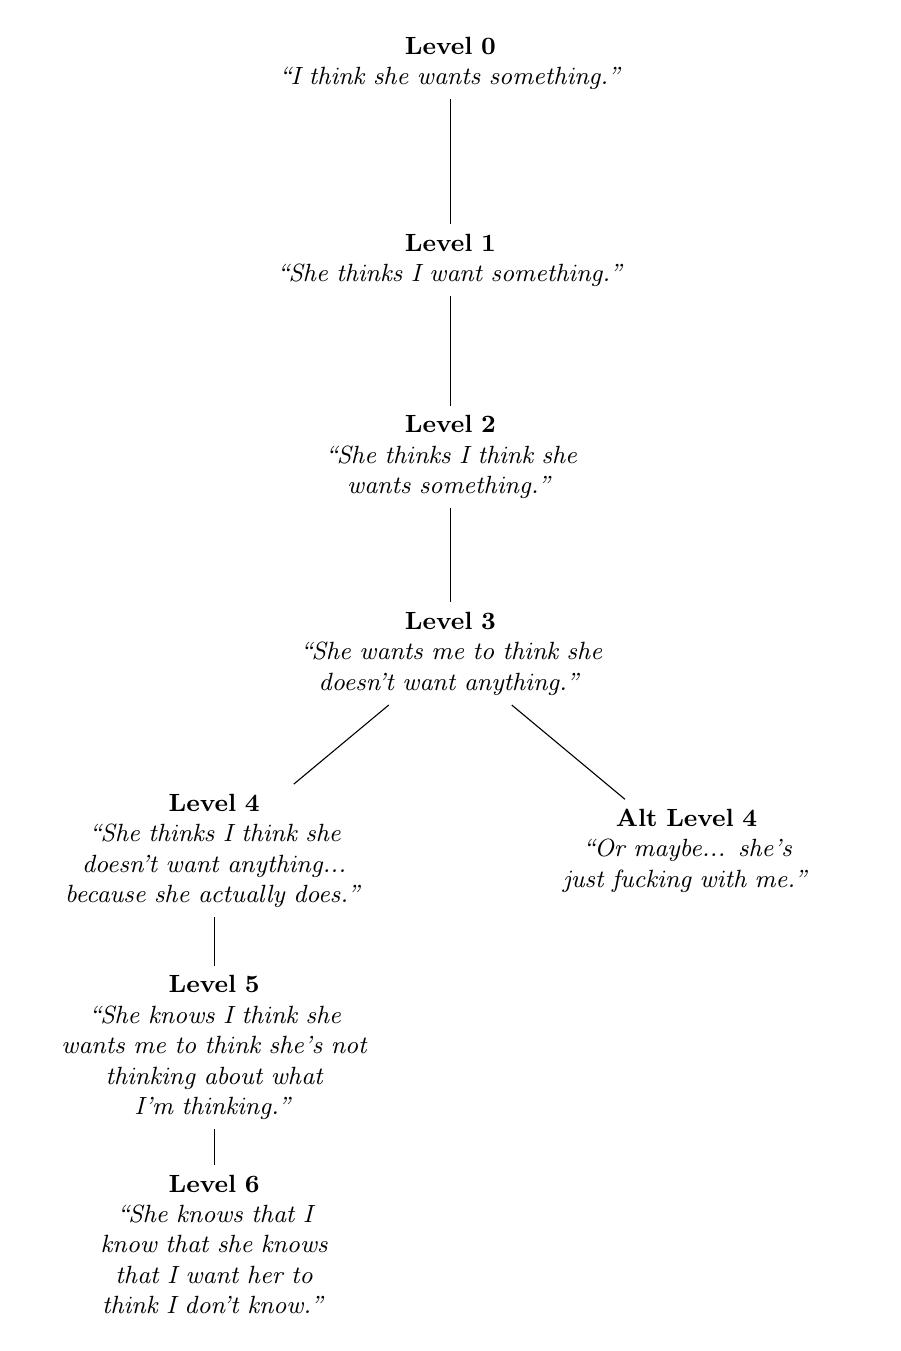
\begin{tikzpicture}[
      level distance=2.5cm,
      level 1/.style={sibling distance=10cm},
      level 2/.style={sibling distance=6cm},
      level 3/.style={sibling distance=4cm},
      level 4/.style={sibling distance=6cm},
      every node/.style={text width=4.5cm, align=center, font=\small}
    ]
    
    \node (root) {\textbf{Level 0}\\\textit{“I think she wants something.”}}
      child { node {\textbf{Level 1}\\\textit{“She thinks I want something.”}} 
        child { node {\textbf{Level 2}\\\textit{“She thinks I think she wants something.”}} 
          child { node {\textbf{Level 3}\\\textit{“She wants me to think she doesn’t want anything.”}} 
            child { node {\textbf{Level 4}\\\textit{“She thinks I think she doesn’t want anything...\\because she actually does.”}} 
              child { node {\textbf{Level 5}\\\textit{“She knows I think she wants me to think she’s not\\thinking about what I’m thinking.”}} 
                child { node {\textbf{Level 6}\\\textit{“She knows that I know that she knows\\that I want her to think I don’t know.”}} }
              }
            }
            child { node {\textbf{Alt Level 4}\\\textit{``Or maybe... she’s just fucking with me.''}} }
          }
        }
      };
    
    \end{tikzpicture}
    \caption{Proof That Grad School Is a Mistake.}
\end{figure}

\medskip

\begin{HistoricalSidebar}{\textbf{John Nash and the Madness of Recursive Models}}

  In the 1950s, mathematician John Nash — pioneer of modern game theory — began suffering from
  paranoid schizophrenia. His delusions weren’t random or chaotic. They were structured.
  Strategic. Often recursive.
  
  \medskip
  
  Nash believed he was receiving secret messages from aliens. That government agents were watching
  him. That he was part of a cosmic game involving hidden codes embedded in newspapers, radio waves,
  and political events.
  
  \medskip
  
  What made Nash’s case so disturbing was not the irrationality — but the rational scaffolding he
  built around it. He used game theory, his own creation, to model the intentions of imagined actors.
  Every silence was a move. Every newspaper headline a signal. Every lack of evidence a clever bluff.
  
  \medskip
  
  In short: his delusion was a closed system of recursive inference. It modeled motives inside
  motives, agents inside agents, until the boundary between truth and simulation collapsed.
  
  \medskip
  
  And yet — remarkably — Nash began to reason his way out.
  
  \medskip
  
  Not by disproving the logic.
  
  \medskip
  
  But by questioning its predictive power.
  
  \medskip
  
  In his own words, he said:
  \textit{``I began to intellectually reject some of the delusionally influenced lines of thinking...
  because they did not lead anywhere.''}
  
  \medskip
  
  Game theory had helped him build a system.But lived experience — and an understanding of epistemic limits — helped him break free.
  
  \medskip
  
  His recovery was not a clean erasure of belief.It was a disciplined decision:To stop believing things simply because they were recursively coherent.
  
  \medskip
  
  As psychologist Dr. Orion Taraban has pointed out: \textit{``Why are beautiful women crazy?''} 
    The answer is unsettlingly simple: \textit{``Because no one tells them the truth.''}
  
  \medskip
  
  When you're surrounded by people who reflect your own projected expectations — whether out of fear, desire,
  or deference — reality becomes recursive. You stop receiving feedback. You start receiving performance.
  
  \medskip
  
  This isn’t limited to relationships. It applies to power.
  Corporate executives fall into the same trap. The higher they climb, the fewer people correct them.
  The fewer people correct them, the more their internal logic ossifies. Soon, strategy collapses
  into simulation — and nobody calls it delusion because the suits are expensive.
  
  \medskip
  
  John Nash’s brilliance made his recursive models sophisticated. But the mechanism wasn’t unique.
  When feedback disappears, anyone — even a Nobel laureate — can get trapped in a loop.
  
  \medskip
  
  \textbf{The danger isn't madness. The danger is insulation.}
  Because once no one tells you the truth, the system you’re modeling stops being the world —
  and starts being you.
  
\end{HistoricalSidebar}

\medskip






Then he started thinking in layers:

\begin{itemize}
    \item \textbf{If Mia was genuine, her restraint was caution.} 
    That would mean she was navigating boundaries delicately — trying not to overstep, trying to stay human. It would imply vulnerability, not strategy.

    \item \textbf{If she wasn’t, her restraint was choreography.} 
    Then every pause, every glance, every omission wasn’t hesitation — it was scripted. A psychological performance designed to evoke trust without revealing intent.

    \item \textbf{If she was following protocol, then the protocol was tuned to his psychology.} 
    That meant he wasn’t being responded to — he was being predicted. Every reaction calibrated in advance, his personality type mapped, modeled, and managed.
\end{itemize}



David had studied multi-level games where agents operated on different time horizons with 
different levels of visibility.
Some players could only see the last move.
Others could see the board and the rules.
A few --- terrifyingly --- could redesign the rules mid-game.

Mia’s silence?
That could be a move.
Or a test.
Or a decoy.

And this elevator?
It wasn’t just an exit.
It was a logging event.

Somewhere, someone might be watching timestamped footage to see how long he hesitated.

David hated how plausible that sounded.

\medskip

\begin{TechnicalSidebar}{Multi-Level Games --- Strategy Across Visibility and Time Horizons}

    In game theory, a \textbf{multi-level game} refers to a strategic environment where agents operate with asymmetries — not just in information, but in power, time, and rules of play.
    
    \medskip
    
    There are typically three structural divides:

    \medskip
    
    \begin{itemize}
        \item \textbf{Visibility:} Some players see only surface-level moves. Others have access to the full board — including intentions, incentives, and constraints. A few may see even beyond that: the agendas of the players themselves.
    
        \item \textbf{Time Horizons:} Some agents optimize for the next move. Others optimize for the next five. Elite players shape the structure so that no matter the moves, the endgame tilts their way.
    
        \item \textbf{Rule Fluidity:} Most players play by the rules. A few — unsettlingly — can edit them. These meta-agents don’t just make moves. They reshape the game space itself.
    \end{itemize}
    
    \medskip
    
    \textbf{Application:} In social and institutional systems, these layers manifest as:

    \medskip
    
    \begin{itemize}
        \item An employee making a decision based on stated policy.
        \item A manager who knows which policies are enforced and which are performative.
        \item An executive who knows when the policy will change — and why.
    \end{itemize}
    
    \medskip
    
    In David’s world, even a pause in front of an elevator could signal intent.  
    Not because of what it was.  
    But because of what it could be interpreted to mean — by someone watching the game from a higher tier.
    
\end{TechnicalSidebar}

\medskip

But David's framing was wrong.

There was no test.

There was no bait.

There was just... proximity.

He hadn’t been asked to compromise.

He hadn’t been offered a bribe.

He hadn’t been promised anything, really.

He was just being offered access.

He was Just being offered attention.

He was just being offered possibility.

David wasn't being pressured. 

\textbf{He was being invited.}

Every event wasn’t a trap. It was an opening.

Every rooftop cocktail wasn’t a test. It was a preview.  

Every afterparty wasn’t a lure. It was a demo.  

Every invitation wasn’t an obligation. It was an opt-in.

No one pushed him. 

No one coerced him. 

No one wanted to. 

Because the club only worked if people \textit{wanted} to join.

And that was the brilliance of it:

\begin{quote}
The lifestyle didn’t recruit.  
The lifestyle didn’t pitch.  
The lifestyle didn’t sell.  
The lifestyle simply made sure you saw what was available.  
And waited for you to ask.
\end{quote}

\begin{PsychologicalSidebar}{The Psychology of Normalization --- How Deviance Becomes ``Just Business''}

  In 1996, sociologist \textbf{Diane Vaughan} coined the term \emph{normalization of deviance} to explain how 
  organizations gradually come to accept risky or unethical practices as routine.

  \medskip
  
  Vaughan’s insight emerged from studying NASA’s Challenger disaster. Engineers had raised concerns about the 
  shuttle’s O-ring failures, but because no catastrophic failure had yet occurred, each overlooked warning became 
  a precedent for tolerating the next. What began as an exception quietly became the norm.

  \medskip
  
  The same psychological drift happens in professional networks.

  \medskip
  
  Each private dinner, each off-the-record conversation, each “minor” regulatory favor lowers the boundary a little more. 
  Individually, no step feels scandalous. But cumulatively, the distance from original ethical standards becomes profound.

  \medskip
  
  \textbf{Albert Bandura’s} theory of \emph{moral disengagement} adds another layer: people rationalize unethical acts by 
  diffusing responsibility, minimizing harm, or reframing misconduct as serving a greater goal.

  \medskip
  
  At Centauri’s table, Aurora’s founders weren’t bribed or threatened. They were absorbed into 
  a culture where favors felt like relationship maintenance, and where blurred lines felt like professional trust.
  
  \begin{quote}
  The brilliance of the system wasn’t coercion.  The brilliance was that by the time you noticed, you didn’t feel trapped.  
  You felt included.
  \end{quote}
  
\end{PsychologicalSidebar}

\medskip

What David hadn’t considered ---
at least not fully ---
was that maybe none of this was centered on him at all.

Maybe he wasn’t the mark.
Maybe he wasn’t the player.
Maybe he wasn’t even on the board.

Maybe Mia’s signal wasn’t a signal.
Maybe it was ambient.
Or directed elsewhere.
Or already spent.

Maybe the timing wasn’t calibrated to him.

Maybe he just happened to be standing in the blast radius.

Because in systems like this,
not every move is strategic.

Some moves are structural.

Some moves are pre-scripted.

And some moves are just... moves.

David thought he was parsing the game.

But he never asked the deeper questions:

\begin{itemize}
    \item What if the asymmetric information wasn't his to overcome?
    \item What if the multiple actors weren’t competing for his attention?
    \item What if he wasn’t playing the game?
    \item What if he was the input?
\end{itemize}

\begin{TechnicalSidebar}{Recursive Reasoning and Common Knowledge in Strategic Environments}

    In multi-agent systems—whether financial, political, or interpersonal—players often operate 
    not just on what they know, but on what they \emph{believe others believe}.

    \medskip
    
    This is called \textbf{recursive reasoning}, and it forms the backbone of higher-order strategy.
    
    \medskip
    
    At level 0, a player responds to direct incentives.  
    At level 1, a player reasons about how others will behave.  
    At level 2, a player reasons about how others believe \emph{they} will behave.  
    And so on—creating a stack of beliefs about beliefs.

    \medskip
    
    This stack doesn’t go infinitely deep in practice.  
    But in high-stakes environments—like negotiations, boardroom politics, or intelligence games—
    even shallow recursion can produce profoundly different outcomes.
    
    \medskip
    
    \textbf{Common knowledge} is a related concept.  
    A fact is common knowledge if:

    \medskip

    \begin{itemize}
        \item Everyone knows it.
        \item Everyone knows that everyone knows it.
        \item Everyone knows that everyone knows that everyone knows it.
    \end{itemize}

    \medskip
    
    Why does this matter?

    \medskip
    
    Because strategy often depends not on facts alone, but on the shared \emph{structure of belief}.  
    In environments with asymmetric information, recursive reasoning becomes essential to detect 
    deception, anticipate reactions, or predict coordination.
    
    \medskip
    
    In David’s case, he initially believed he was the analyst:
    interpreting Mia’s behavior, evaluating hidden incentives, and mapping possible games.

    \medskip
    
    But recursive reasoning cuts both ways.

    \medskip
    
    What David didn’t realize was that his reactions—his hesitations, his framing, even his 
    overanalysis—could themselves be \emph{the object of observation}.
    
    \begin{quote}
    Recursive environments don’t just reward strategy.
    
    They harvest it.
    \end{quote}
    
\end{TechnicalSidebar}


